%\chapter{Pierwszy dokument}
%\label{cha:pierwszyDokument}
%
%W rozdziale tym przedstawiono podstawowe informacje dotyczące struktury prostych plików \LaTeX a. Omówiono również metody kompilacji plików z zastosowaniem programów \emph{latex} oraz \emph{pdflatex}.
%
%%---------------------------------------------------------------------------
%
%\section{Struktura dokumentu}
%\label{sec:strukturaDokumentu}
%
%Plik \LaTeX owy jest plikiem tekstowym, który oprócz tekstu zawiera polecenia formatujące ten tekst (analogicznie do języka HTML). Plik składa się z dwóch części:
%\begin{enumerate}%[1)]
%\item Preambuły -- określającej klasę dokumentu oraz zawierającej m.in. polecenia dołączającej dodatkowe pakiety;
%
%\item Części głównej -- zawierającej zasadniczą treść dokumentu.
%\end{enumerate}
%
%
%\begin{lstlisting}
%\documentclass[a4paper,12pt]{article}      % preambuła
%\usepackage[polish]{babel}
%\usepackage[utf8]{inputenc}
%\usepackage[T1]{fontenc}
%\usepackage{times}
%
%\begin{document}                           % część główna
%
%\section{Sztuczne życie}
%
%% treść
%% ąśężźćńłóĘŚĄŻŹĆŃÓŁ
%
%\end{document}
%\end{lstlisting}
%
%Nie ma żadnych przeciwskazań do tworzenia dokumentów w~\LaTeX u w~języku polskim. Plik źródłowy jest zwykłym plikiem tekstowym i~do jego przygotowania można użyć dowolnego edytora tekstów, a~polskie znaki wprowadzać używając prawego klawisza \texttt{Alt}. Jeżeli po kompilacji dokumentu polskie znaki nie są wyświetlane poprawnie, to na 95\% źle określono sposób kodowania znaków (należy zmienić opcje wykorzystywanych pakietów).
%
%
%%---------------------------------------------------------------------------
%
%\section{Kompilacja}
%\label{sec:kompilacja}
%
%
%Załóżmy, że przygotowany przez nas dokument zapisany jest w pliku \texttt{test.tex}. Kolejno wykonane poniższe polecenia (pod warunkiem, że w pierwszym przypadku nie wykryto błędów i kompilacja zakończyła się sukcesem) pozwalają uzyskać nasz dokument w formacie pdf:
%\begin{lstlisting}
%latex test.tex
%dvips test.dvi -o test.ps
%ps2pdf test.ps
%\end{lstlisting}
%%
%lub za pomocą PDF\LaTeX:
%\begin{lstlisting}
%pdflatex test.tex
%\end{lstlisting}
%
%Przy pierwszej kompilacji po zmiane tekstu, dodaniu nowych etykiet itp., \LaTeX~tworzy sobie spis rozdziałów, obrazków, tabel itp., a dopiero przy następnej kompilacji korzysta z tych informacji.
%
%W pierwszym przypadku rysunki powinny być przygotowane w~formacie eps, a~w~drugim w~formacie pdf. Ponadto, jeżeli używamy polecenia \texttt{pdflatex test.tex} można wstawiać grafikę bitową (np. w formacie jpg).
%
%
%
%%---------------------------------------------------------------------------
%
%\section{Narzędzia}
%\label{sec:narzedzia}
%
%
%Do przygotowania pliku źródłowego może zostać wykorzystany dowolny edytor tekstowy. Niektóre edytory, np. GEdit, mają wbudowane moduły ułatwiające składanie tekstów w LaTeXu (kolorowanie składni, skrypty kompilacji, itp.).
%
%Jednym z bardziej znanych środowisk do składania dokumentów  \LaTeX a jest {\em TeXstudio}, oferujące kompletne środowisko pracy. Zobacz: \url{http://www.texstudio.org}
%
%
%Bardzo dobrym środowiskiem jest również edytor gEdit z wtyczką obsługującą \LaTeX a. Jest to standardowy edytor środowiska Gnome. Po instalacji wtyczki obsługującej \LaTeX~ zamienia się w wygodne i szybkie środowisko pracy.
%
%\textbf{Dla testu łamania stron powtórzenia powyższego tekstu.}
%
%
%Do przygotowania pliku źródłowego może zostać wykorzystany dowolny edytor tekstowy. Niektóre edytory, np. GEdit, mają wbudowane moduły ułatwiające składanie tekstów w LaTeXu (kolorowanie składni, skrypty kompilacji, itp.).
%Jednym z bardziej znanych środowisk do składania dokumentów  \LaTeX a jest {\em TeXstudio}, oferujące kompletne środowisko pracy. Zobacz: \url{http://www.texstudio.org}
%Bardzo dobrym środowiskiem jest również edytor gEdit z wtyczką obsługującą \LaTeX a. Jest to standardowy edytor środowiska Gnome. Po instalacji wtyczki obsługującej \LaTeX~ zamienia się w wygodne i szybkie środowisko pracy.
%Po instalacji wtyczki obsługującej \LaTeX~ zamienia się w wygodne i szybkie środowisko pracy.
%
%Do przygotowania pliku źródłowego może zostać wykorzystany dowolny edytor tekstowy. Niektóre edytory, np. GEdit, mają wbudowane moduły ułatwiające składanie tekstów w LaTeXu (kolorowanie składni, skrypty kompilacji, itp. itd. itp.).
%Jednym z bardziej znanych środowisk do składania dokumentów  \LaTeX a jest {\em TeXstudio}, oferujące kompletne środowisko pracy. Zobacz: \url{http://www.texstudio.org}
%Bardzo dobrym środowiskiem jest również edytor gEdit z wtyczką obsługującą \LaTeX a. Jest to standardowy edytor środowiska Gnome. Po instalacji wtyczki obsługującej \LaTeX~ zamienia się w wygodne i szybkie środowisko pracy.
%
%Do przygotowania pliku źródłowego może zostać wykorzystany dowolny edytor tekstowy. Niektóre edytory, np. GEdit, mają wbudowane moduły ułatwiające składanie tekstów w LaTeXu (kolorowanie składni, skrypty kompilacji, itp.).
%Jednym z bardziej znanych środowisk do składania dokumentów  \LaTeX a jest {\em TeXstudio}, oferujące kompletne środowisko pracy. Zobacz: \url{http://www.texstudio.org}
%Bardzo dobrym środowiskiem jest również edytor gEdit z wtyczką obsługującą \LaTeX a. Jest to standardowy edytor środowiska Gnome. Po instalacji wtyczki obsługującej \LaTeX~ zamienia się w wygodne i szybkie środowisko pracy.
%
%%---------------------------------------------------------------------------
%
%\section{Przygotowanie dokumentu}
%\label{sec:przygotowanieDokumentu}
%
%Plik źródłowy \LaTeX a jest zwykłym plikiem tekstowym. Przygotowując plik
%źródłowy warto wiedzieć o kilku szczegółach:
%
%\begin{itemize}
%\item
%Poszczególne słowa oddzielamy spacjami, przy czym ilość spacji nie ma znaczenia.
%Po kompilacji wielokrotne spacje i tak będą wyglądały jak pojedyncza spacja.
%Aby uzyskać {\em twardą spację}, zamiast znaku spacji należy użyć znaku {\em
%tyldy}.
%
%\item
%Znakiem końca akapitu jest pusta linia (ilość pusty linii nie ma znaczenia), a
%nie znaki przejścia do nowej linii.
%
%\item
%\LaTeX~sam formatuje tekst. \textbf{Nie starajmy się go poprawiać}, chyba, że
%naprawdę wiemy co robimy.
%\end{itemize} 
%
%



% ############# ROZDZIAŁ 2 ###############
\chapter{Stan badań}
\label{cha:cha2}

\section{Powiązane prace – zarys historyczny}
\subsection{Predykcja wartoci liczby ferrytowej}

Przewidywanie własności mechanicznych produktów odlewniczych za pomocą metod uczenia maszynowego ma niemal tak długą historię, jak sama dziedzina uczenia maszynowego. Już w jednej z pierwszych prac naukowych na ten temat [3] (1985) mówiono o tym, że przyszłe techniki predykcyjne będą opierać się raczej na wyrażeniach matematycznych czy sztucznej inteligencji niż na diagramach. 
Ówcześnie do przewidywania fazy mikrostruktury spoiny metalu wykorzystywano właśnie diagramy (rys. 1), lecz jak łatwo się domyślić, jest to podejście mało praktyczne. Stąd nacisk na wykorzystywanie jak najbardziej wszechstronnych wyrażeń ilościowych do przewidywania mikrostruktury jako funkcji m.in. składu.

\begin{figure}[h]
    \centering
    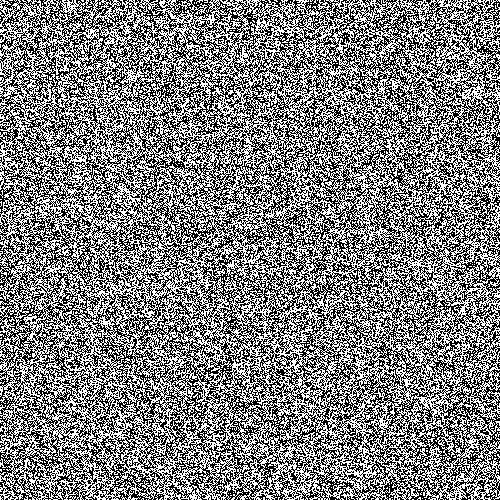
\includegraphics[width=1\textwidth]{rys.1.WRC.Delong.png}
    \caption{Przykładowy schemat do wyznaczania ferrytu $ \delta $ z granicami składu (DeLong, 1973)}
    \label{fig:mesh1}
\end{figure}

Następnym krokiem było opracowanie modelu półempirycznego w celu powiązania składu metalu spoiny z liczbą ferrytową (zwaną dalej FN), czyli miarą oznaczania zawartości ferrytu w stali nierdzewnej. Dlaczego jest to istotne? Jak wskazano w pracy [7] wielkość FN określa właściwości metalu takie, jak wytrzymałość, twardość, odporność na korozję i inne (jej poziom powinien wynosić 3-7\%, ponieważ niski poziom ferrytu może prowadzić do pęknięć [4, 6], z drugiej strony wysoki poziom ferrytu prowadzi do niższej odporności na korozję [6]). 
W pracy Babu i in. [5] (1997) przedstawiono wyniki aproksymacji punktowej, która dopasowuje model do prognoz zgodnych z obserwacjami eksperymentalnymi. Stwierdzono w niej, iż ogólna dokładność badanego modelu jest porównywalna do tej z diagramu WRC 1992 (czyli najnowocześniejszej ówcześnie metody – przyp. aut.), który powstał w ten sposób, iż skład stopu jest konwertowany do dwóch czynników – ekwiwalentu chromu ($Cr_{eq}$, wzór 1) oraz ekwiwalentu niklu ($Ni_{eq}$, wzór 2). Wynika to z tego, iż ten pierwszy zawiera elementy, które wpływają na mikrostrukturę w ten sam sposób jak chrom (tj. stabilizatory ferrytu), natomiast ten drugi zawiera elementy, które wpływają na mikrostrukturę w ten sam sposób, jak nikiel (tj. stabilizatory austenitu). Następnie z diagramu można odczytać poziom ferrytu, który jest przedstawiony jako funkcja od ekwiwalentów chromu i niklu. Jak stwierdzają autorzy [5], zaletą aproksymacji punktowej w porównaniu z diagramem WRC 1992 jest jego zdolność do uwzględniania wpływu innych pierwiastków stopowych oraz łatwość ekstrapolacji do wyższych wartości $Cr_{eq}$ i $Ni_{eq}$ (WRC 1992 jest pod tym względem mocno ograniczone, co widać na rysunku 2).

\begin{figure}[h]
    \centering
    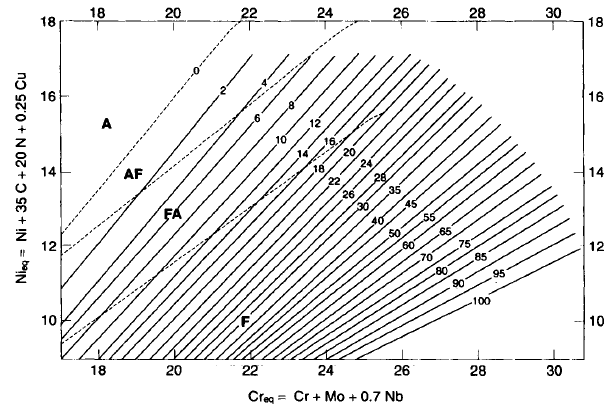
\includegraphics[width=1\textwidth]{rys.2.WRC.Kotecki.png}
    \caption{Diagram WRC 1992 (Kotecki \& Siewert, 1992)}
    \label{fig:mesh2}
\end{figure}

Równania na  $Cr_{eq}$ i $Ni_{eq}$ są następujące:

\begin{equation}
Cr_{eq} = Cr + Mo + 0.7Nb
\end{equation}
% Wzór na ekwiwalent Chromu w diagramie WRC-1992

\begin{equation}
Ni_{eq} = Ni+35C+20N+0.25Cu
\end{equation}
%Wzór na wartość ekwiwalentu Niklu w schemacie WRC-1992

gdzie symbole pierwiastków przedstawiają procent wagi każdego pierwiastka.
W kolejnej pracy [7] dotyczącej predykcji FN ci sami autorzy wykorzystali sieć neuronową, która na wejściu przyjmowała procent wagowy 13 pierwiastków (Fe, Cr, Ni, C, N, Mo, Mn, Si, Cu, Ti, Nb, V i Co), czyli warstwa z 13 neuronami, następnie warstwa ukryta z sześcioma neuronami, natomiast na wyjściu był pojedynczy neuron, który zwracał liczbę ferrytową (rys. 3).

\begin{figure}[h]
    \centering
    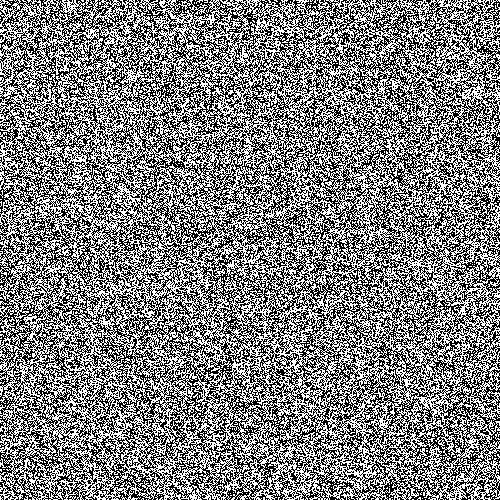
\includegraphics[width=1\textwidth]{rys.3.ORFN.Vitek.2003.png}
    \caption{Model sieci neuronowej ORFN (Vitek, 2003)}
    \label{fig:mesh3}
\end{figure}

Wyniki zostały przedstawione w [8] i jak się okazało, testowana sieć zwracała lepsze wyniki od jakichkolwiek dotychczasowych podejść z błędem RMS mniejszym o 50\% od poprzedniej najlepszej metody. 
    W ostatnim przytoczonym artykule dotyczącym predykcji FN [9] również zastosowano sieć neuronową, a konkretnie bayesowską sieć neuronową (BNN). Na wejściu mamy taką samą warstwę, jak w poprzedniej pracy, natomiast tutaj jest więcej neuronów w warstwie ukrytej. Poprawa wyników względem poprzedniej pracy wynosi około 15\% (błąd RMS) testując na niezależnym zbiorze danych nieużywanym w szkoleniu.

\subsection{Predykcja własności mechanicznych odlewów}

Początki rozwoju i przetwarzania materiałów nie były łatwe. Mimo wielu przeprowadzonych badań naukowych nad materiałami wciąż pozostaje wiele problemów, w przypadku których brakuje metod ilościowych. Tyczy się to głównie predykcji takich parametrów konstrukcyjnych jak wytrzymałość na rozciąganie, trwałość, twardość itp. Pierwsze badania dotyczące własności mechanicznych odlewów przyjmujące podejście ilościowe brały pod uwagę szczegółowy skład chemiczny oraz takie parametry jak rekrystalizacja, proces starzenia, zakres pracy na zimno, temperatura badania czy szybkość odkształcania [10, 11]. W obydwu tych pracach zastosowano sieci neuronowe oraz uzasadniono, że modele matematyczne sobie nie radzą z wymienionymi wyżej parametrami. Standardowo zastosowano sieć, w której na wejściu podawano procent wagowy pierwiastków w badanym materiale. 
Jedną z głównych własności mechanicznych jest wytrzymałość na rozciąganie (ang. ultimate tensile strength, UTS), która jest badana od wielu lat. Po fazie odlewu inżynierowie wykorzystują w swoich obliczeniach tę i inne wartości w celu obliczenia odkształcania się, funkcji przyłożonego obciążenia, czasu i wiele innych. Jest ona jednym z ważniejszych czynników do uwzględnienia, gdyż niewystarczająca wartość wytrzymałości może mieć fatalne skutki (jak np. zawalenie się konstrukcji). Innym powodem może być to, iż jedynym sposobem, aby zbadać wartość tej wytrzymałości trzeba przeprowadzić badania niszczące, co powoduje wzrost kosztów produkcji [1]. Jednym ze sposobów analizy wartości UTS jest predykcja za pomocą wartości różnych właściwości odlewu. W przywołanej wcześniej pracy [1] oraz [12] są to skład chemiczny, rozmiar odlewu, prędkość chłodzenia, obróbka termiczna. Mając dane w postaci CSV (wartości rozdzielone przecinkiem, od ang. comma-separated values) można skorzystać z klasycznych metod klasyfikacji statystycznej, jak klasyfikacja liniowa, K-najbliższych sąsiadów, drzewa decyzyjne, czy sieci bayesowskie [2]. W przytoczonej pracy skupiono się na sieciach bayesowskich. Wyniki są optymistyczne: dokładność na poziomie ponad 82\% oraz błędy MAE (średni błąd bezwzględny, od ang. mean absolute error) oraz MSE (średni błąd kwadratowy, od ang. mean square error) na poziomie odpowiednio 0.2 oraz 0.35. Inne przetestowane metody w tym artykule to KNN (k najbliższych sąsiadów, od ang. k-Nearest Neighbors) oraz ANN (sztuczne sieci neuronowe, od ang. artificial neural networks), które osiągnęły podobne, aczkolwiek nieco gorsze wyniki. 
Wytrzymałość na rozciąganie można przewidzieć na podstawie dwóch różnych źródeł danych wejściowych [13]:
1) skład chemiczny metalu oraz zmienne procesu walcowania, jak temperatura, czy przebieg;
2) dane na temat mikrostruktury. 
W pracy tej jako dane wejściowe użyto skład chemiczny, specyfikacje geometryczne oraz zmienne dotyczące procesu rolowania, natomiast modelem wykorzystanym do predykcji wartości wytrzymałości na rozciąganie była ponownie bayesowska sieć neuronowa. Sieć ta składała się z jednej warstwy ukrytej, która z kolei składała się z siedmiu neuronów. Jak stwierdzają autorzy, sieć BNN lepiej się sprawdza w tym celu od tradycyjnych sieci neuronowych, a to ze względu na wyższą odporność na nadmierne dopasowanie danych (overfitting), szczególnie w przypadku, gdy ilość danych jest znacznie ograniczona i nie mamy możliwości zgromadzenia dużej ilości wysokiej jakości danych.
    Bardzo podobne podejście zastosowano w pracy [19], gdzie użyto sieci neuronowej, a na jej wejściu podawano 20 zmiennych, takich jak skład chemiczny, warunki obróbki cieplnej czy temperatura badania. W ten sposób uzyskano 93\% wartości współczynnika R-kwadrat dla YS oraz UTS.
















